\begin{comment}
Fragestellung:
- Welche elektrische Beschaltung ist notwendig um das DWM1000 Modul von DecaWave in Betrieb nehmen zu können?
- Wie erfolgt die Entfernungsmessung zwischen den einzelnen UWB--Modulen?
- Wie erfolgt der Datenaustausch zwischen einem UWB--Modul und der Verarbeitungseinheit?
\end{comment}

\begin{comment}
------------------------------------------------------------------------------------------
Schmalbandkommunikation (engl. Narrowband)
Frequenzband (engl. Radio spectrum)
Frequenzspreizung (engl. spread spectrum)
Basisband (engl. Baseband)
https://en.wikipedia.org/wiki/Ultra-wideband
\end{comment}
\chapter{\acrlong{uwb}}

Bei der normalen Funkübertragung werden die zu übermittelnden \Gls{basisband}signale auf eine sinusförmige Trägerfrequenz aufmoduliert. Bei der \Gls{uwb}--Übertragung ist das nicht der Fall, die Signale werden im \Gls{basisband} übertragen. Hierfür werden im Nanosekunden--Bereich kurze Impulse erzeugt. \Gls{uwb}--Signale verwenden eine Bandbreite von bis zu \SI{500}{\MHz} und können im Frequenzbereich von \SIrange{3.6}{10.1}{\GHz} eingesetzt werden. Um zu verhindern das bestehende Dienste wie \Gls{gps} oder \Gls{wlan} gestört werden, wurde durch die \Gls{fcc} die maximale Abgabeleistung von \Gls{uwb}--Sendern stark begrenzt (unter \SI[per-mode=symbol]{-41.3}{\dBm\per\MHz}). Dadurch ist eine Koexistenz mit den bereits bestehenden Diensten möglich, ohne das diese sich gegenseitig stören. \cite{win1998impulse, yang2004uwbcom, fontana2004recent, aiello2006ultra, yavari2014ultra}

Zu den bemerkenswerten Eigenschaften der \Gls{uwb}--Technologie zählt das verlustfreie Durchdringen von Hindernissen, präzise Entfernungsmessung im Zentimeterbereich, eine hohe Datenübertragungsrate von über \SI[per-mode=symbol]{110}{\mega\byte\per\second} in einem Bereich von \SIrange{10}{15}{\metre} und der geringe Energieverbrauch. \cite{yang2004uwbcom}

Die Einsatzgebiete werden dabei in die Klassen Bildgebene--, Kommunikation--, Mess-- und Fahrzeugradarsysteme unterteilt. Der Bereich der Bildgebenensysteme ist weiter unterteilt in Bodenradar, Medizinische Überwachung und Diagnostik und in Überwachungsysteme die Objekte durch Wände erkennen können. Kommunikations-- und Messsysteme werden ihrerseit unterteilt in Indoor-- und Outdoor--Systeme unterweilt. Hierzu zählen auch Systeme für die Navigation, Güternachverfolgung und Hochgeschwindigkeitsdatenübertragung. Die letzte Klasse wird in die Bereiche der Kollisionsvermeidung und Abstandssysteme unterteilt. \cite{yang2004uwbcom, lakkundi2006ultra, pan2007medical}


\begin{comment}
------------------------------------------------------------------------------------------
\end{comment}
\section{Historie}

Als Vater der \gls{uwb} Kommunikation kann der italienische Funkpionier Guglielmo Marconi angesehen werden. In den späten 1890er Jahren entwickelte er den Knallfunkensender, der über eine Funkenstrecke ein hochfrequentes Signal zur Übertragung von Morsezeichen erzeugt. Mit dieser Apparatur gelang es Ihm, im Jahre 1901 einen Nachrichtenaustausch zwischen Nordamerika und Europa über den Nordatlantik durchzuführen.\cite{fontana2004recent}

% Weitere Quellen:
% http://www.ieee.ca/millennium/radio/radio_differences.html
% https://de.wikipedia.org/wiki/Knallfunkensender

Bis in die Anfänge der 1960er Jahre dominierte jedoch die sinusförmige Funkübertragungsform. Dies änderte sich als die Forscher vom \gls{llnl} und \gls{lanl} begangen die Ausbreitung elektromagnetischer Wellen nicht zur im Frequenz- sondern auch im Zeitbereich zu untersuchen. Grundlegende Erkenntnisse wurden dabei im Bereich der Impulssender, -empfänger und -antennen gesammelt.\cite{eltaher2004positioning, fontana2004recent, lakkundi2006ultra, aiello2006ultra}

% TODO: time-domain sampling oscilloscopes
Durch die Einführung der zeitbereichs basierten Abtast--Oszilloskope im Jahre 1962 durch Tektronix bzw. Hewlett-Packard war es zum ersten Mal möglich eine \gls{uwb} Wellenform aufzufangen und anzuzeigen. Ermöglicht wurde dies erst durch den Einsatz von Tunneldioden und Avalanchetransistoren. \cite{fontana2004recent, lakkundi2006ultra, aiello2006ultra}

Ab dem Jahre 1964 produzierten beide Hersteller Messgeräte für die Diagnose im Zeitbereich. \cite{barrett2001technical}

Ab den Anfängen der 1970er Jahre waren alle wichtigen Grundsteine für ein \gls{uwb} System für Kommunikation- bzw. Radaranwendungen gelegt. Dazu zählten auch diverse eingereichte Patente von Harmuth an der \gls{cua}, Ross und Robbins bei der Sperry Rand Corporation und Paul van Etten an der \gls{usaf} im Rome Air Development Center.\cite{barrett2001technical, fontana2004recent, yang2004uwbcom} Hervorzuheben ist das eingereichte Patent von Ross im Jahre 1973, siehe \cite{g1973transmission}.

% INFO:
% Rome Laboratory (Rome Air Development Center until 1991) is the US
% "Air Force 'superlab' for command, control, and communications"[4] research and
% development and is responsible for planning and executing the USAF science and
% technology program.

% TODO: Warum ist gerade diese Patent hervorzuheben?
% US 3728632 A
% Transmission and reception system for generating and receiving base-band pulse
% duration pulse signals without distortion for short base-band communication system
% Veröffentlichungsnummer: US3728632 A
% Publikationstyp: Erteilung
% Veröffentlichungsdatum	: 17. Apr. 1973
% Eingetragen: 12. März 1971
% Erfinder:	Ross G
% Ursprünglich Bevollmächtigter: Sperry Rand Corp
% ZUSAMMENFASSUNG
% An electromagnetic signal communication system utilizing short base-band pulse
% signals of sub-nanosecond duration employs dispersionless, broad band antenna
% transmission line elements for generating and preserving the character of the
% short base-band pulses in respective transmitter and receiver sub-systems.

Kurz darauf im Jahre 1974 wurde die \gls{uwb} Technologie kommerziell erfolgreich von Morey bei der \gls{gssi} für ein Bodenradar (engl. \acrfull{gpr}) angewendet. \cite{barrett2001technical}

Im Zeittraum von 1977 is 1989 wurden mehrere Programme und Workshops organisiert um die Entwicklung von \gls{uwb} Systemen voranzutreiben, darunter auch bei der \gls{usaf} und dem \gls{usdod}. Ebenfalls gabe es mehrere akademische Programme an diversen Instituten, darunter auch am \gls{llnl}, \gls{lanl}, University of Michigan, University of Rochester und
Polytechnic University, mit dem Fokus auf den physikalischen Unterschieden zwischen der Kurzimpulsübertragung und den Langimpulssignalen bzw. kontinuierlichen Impulssignalen bei der Interaktion mit verschiedenen Materialien.\cite{barrett2001technical}

% TODO: Der letzte Satz ist zu lang. Aufspalten!

Ab dem Jahre 1989 wurde der Name \gls{uwb} durch das \gls{usdod} geprägt. Diese Definition galt für alle Geräte die mindestens eine Bandbreite von \SI{1.5}{\GHz} bzw. \SI{25}{\percent} der \gls{fbw} belegten. Vorher war die \gls{uwb} Technologie nur unter den Synonymen ``baseband communication'', ``carrier free communication'', ``impulse radio'', ``large relative bandwidth communication'', ``nonsinusoidal communication'', ``orthogonal functions'', ``sequency theory'', ``time domain'', ``large-relative-bandwidth radio/radar signals'', ``video-pulse transmission'' und/oder ``Walsh waves communication'' bekannt. \cite{eltaher2004positioning, fowler1990assessment, yang2004uwbcom, aiello2006ultra, fontana2004recent}

% TODO: Fachbegriffe Übersetzen?

% TODO: Sollen die Militärischen Anwendungfälle erwähnt werden? Vielleicht besser bei der FCC regulierung.
% Das Militär hatte dabei für sich die Anwendungsfälle im Bereich Radar und hochsicherheitskommunkation entdeckt.\cite{eltaher2004positioning}

Im Jahre 1994 wurde von McEwan an der \gls{llnl} das \gls{mir} konstruiert. Hierbei handelte es sich um ein \gls{uwb} Radarsystem mit bemerkenswerten Eigenschaften. Das Radarsystem verfügte über eine sehr hohe Signalsensitivität, einen kompakten Aufbau, eine kostengünstige Herstellung und einen der geringer Energieverbrauch, der sich im Bereich von Mikrowatt befanden und daher ideal für batteriebetriebene Anwendung eignete. \cite{barrett2001technical}

% TODO: Zwei mal bemerkenswerte Eigenschaften. Korrigieren bzw. Umformulieren!!!

Vor dem Jahre 2002 war die Verwendung von \gls{uwb} auf Radarssytem beschränkt, die größtenteils in militärischen Anwendungen aufzufinden waren. \cite{yang2004uwbcom} Das änderte sich ab dem Jahre 1998, als die \gls{fcc} mit der Standardisierung der \gls{uwb} Nutzung begann. Im Jahre 2002 wurden durch die \gls{fcc} in den Vereinigten Staten von Amerika große Frequenzbereiche (\SIrange{3.6}{10.1}{\GHz}) für die kommerzielle Nutzung freigegeben hat, siehe First Report and Order (R\&O). Danach wurden erstmals auch eine nicht militärische Anwendungen im Bereich ``Imaging systems'', ``communication and measurement systems'' und ``vehicular radar systems'' möglich. \cite{yang2004uwbcom}

% TODO: Zitieren des FCC R&O
% [12] FCC First Report and Order: In the matter of Revision of Part 15 of the
% Commission’s Rules Regarding Ultra-Wideband Transmission Systems,
% FCC 02–48, April 2002.
% Chrome: g FCC 02-48 bibtex
% https://transition.fcc.gov/Bureaus/Engineering_Technology/Orders/2002/fcc02048.pdf

Weitere Staten folgten der \gls{fcc} Regulierung/Standardierung und gaben ebenfalls große Frequenzbereiche für die \gls{uwb} Technologie frei. Details zu den Regularien der einzelnen Staten können unter \cite{decawave2015uwbreg} eingesehen werden.

	
\begin{comment}
------------------------------------------------------------------------------------------
- Welche alternativen Technologien gibt es zu UWB?
- Einen guten Überblick über die Eigenschaften der Drahtlosen-Protokolle (engl. Wireless Protocols) Bluetooth, UWB, ZigBee und WiFi liefert die Arbeit \cite{lee2007comparative} von \citeauthor{lee2007comparative}.
	- Bluetooth
		- Piconet/Scatternet
		- low data rate
		- small data sizes (around smaller than 339 bytes)
		- is the most complicated protocol with 188 primitives and events in total
		- intended for portable products, short ranges, and limited battery power.
	- ZigBee
		- supporting simple devices that consume minimal power and typically operate in the personal operating space (POS) of 10m.
		- full-function device (FFD) and a reduced-function device (RFD)
		- low data rate
		- highest transmission time
		- data size smaller than 102 bytes
		- is the simplest one with only 48 primitives
		- the simplicity makes ZigBee very suitable for sensor networking applications due to their limited memory and computational capacity.
		- intended for portable products, short ranges, and limited battery power.
	- UWB
		- Indoor short-range high-speed wireless communication
		- high data rate
		- lowest transmission time
		- large data sizes much better efficiency
		- proposed for shortrange and high data rate applications.
		- have better efficiency in energy consumption.
	- WiFi
		- allows users to surf the Internet at broadband speeds when connected to an access point (AP) or in ad hoc mode.
		- high data rate
		- large data sizes much better efficiency
		- designed for a longer connection and supports devices with a substantial power supply
		- have better efficiency in energy consumption.
- For a wireless sensor network in factory automation systems, since most data size of industrial monitoring and control are generally small, (e.g. the temperature data in an environmental monitoring may required less than 4 bytes only), Bluetooth and ZigBee protocols may be a good selection (from a data coding efficiency point of view) in spite of their slow data rate.
- Welche Eigenschaften haben die alternativen Technologien?
- Warum hab ich mich für UWB entschieden?
\end{comment}
%\section{Alternative Technologien/Gegenüberstellung}


\begin{comment}
------------------------------------------------------------------------------------------
\end{comment}
\section{Erstellte Hardware}

\begin{comment}
------------------------------------------------------------------------------------------
- Datenübertragung zum Host
- Batteriebetrieb
- TODO: Erweiterbare Hardwareplattform
\end{comment}
\subsection{Anforderungen}

An die zu erstellende Hardware werden mehrere Anforderungen gestellt.

Um eine Entfernungsmessung durchzuführen wird immer ein Marker und mindestens ein Anker benötigt. Sowohl der Marker als auch der Anker sollen aus den gleichen elektrischen Komponenten bestehen, also eine gemeinsame Harewareplattform bilden. Die unterschiedliche Funktionalität pro Modul soll sich dann aus verschiedenen Software-Ständen der Firmware herausbilden.

Die Anker sollen im Bedarfsfall frei im Raum verteilt werden können. Nicht an jeder Stelle steht eine Stromversorgung zur Verfügung, daher muss jedes Modul über eine separate Energiequelle verfügen.

Zusätzlich muss der Marker über eine bidirektional Kommunikationsschnittstelle zur Verarbeitungseinheit verfügen. Über diese sollen zum einen Steuerbefehle an das UWB--Modul geschickt werden und zum anderen sollen die gemessenen Entfernungen zwischen dem Marker und den Ankern an die Verarbeitungsanleitung übertragen werden.


\begin{comment}
------------------------------------------------------------------------------------------
- Zusätzlich werden Erfahrungsberichte aus dem Internet ausgewertet um die Beschaltung weiter zu verfeinern, siehe \cite{Trojer2015, Holder2016, Holder2016a}.
\end{comment}
\subsection{Hardware Zusammenstellung}


\begin{comment}
------------------------------------------------------------------------------------------
TODO: Wie wird der Vorwiderstand berechnet? ca. 10mA bei 1.8V, R=(U_0-U_LED)/I_LED

LED Vorwiderstand berechnen
	- https://www.youtube.com/watch?v=iNZj91TSRUg
	- DW1000 Datasheet - 5.9 General Purpose Input Output (GPIO)
\end{comment}
\subsubsection{\gls{uwb}--Transceiver}\label{subsec:uwb_transceiver}

Als \gls{uwbt} werden die Komponenten der Firma DecaWave verwendet. Bei dem DW1000 handelt es sich nur um dem \gls{ic} der für die Erzeugen und Verarbeiten der \gls{uwb}--Funksignale zuständig ist. Der DWM1000 beinhaltet neben dem DW1000 auch die notwendige Beschaltung und zusätzlich eine Antenne für die Übertragung, siehe \figurename~\ref{fig:pin_assignment}.

\begin{figure}
	\begin{subfigure}[t]{0.4\textwidth}
		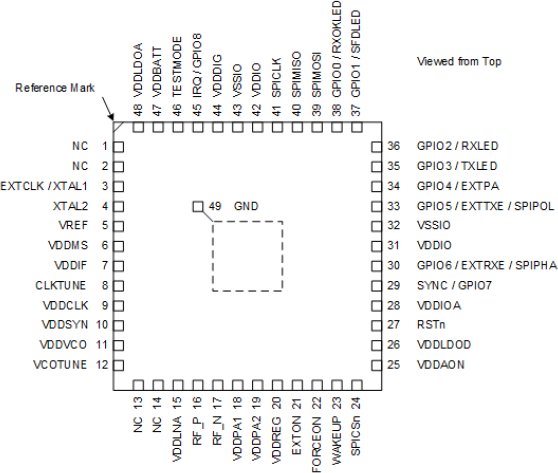
\includegraphics[width=\textwidth]{dw1000_pin_assignments.png}
		\caption{DW1000 \gls{ic}}
		\label{fig:dw1000_pin_assignments}
		\source{\cite{decawave2016dw1kdatasheet}}
	\end{subfigure}
	\hfill
	\begin{subfigure}[t]{0.4\textwidth}
		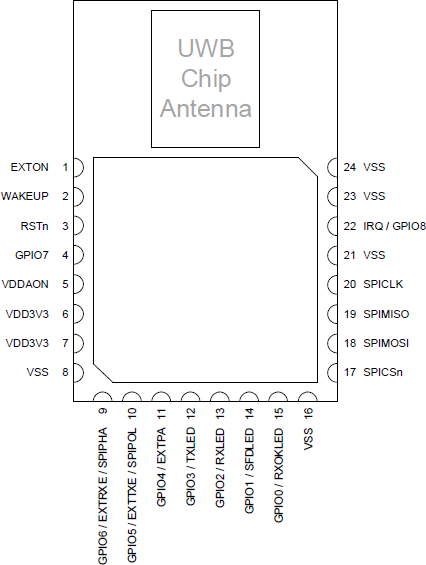
\includegraphics[width=\textwidth]{dwm1000_pin_assignments.png}
		\caption{DWM1000 Modul}
		\label{fig:dwm1000_pin_assignments}
		\source{\cite{decawave2016dwm1kdatasheet}}
	\end{subfigure}
	\caption{DecaWave \gls{ic} Pin Belegung}
	\label{fig:pin_assignment}
\end{figure}

Der DWM1000 kann mit einer Spannung von \SIrange{2.8}{3.6}{\volt}\cite{decawave2016dwm1kdatasheet} betrieben werden, idealerweise mit \SI{3.3}{\volt}. Das bedeutet aber auch, dass die Logikpegelspannung für die \gls{spi} Schnittstelle \SI{3.3}{\volt} beträgt. Dieser Umstand muss bei der Auswahl des Mikrocontrollers berücksichtig werden.

Die Kommunikation mit dem DWM1000 erfolgt über die \gls{spi} Schnittstelle, hierfür sind die Pins \gls{sclk}, \gls{mosi}, \gls{miso} und \gls{ss} zu verwenden \cite{decawave2016dwm1kdatasheet}. Bei der \gls{spi}--Schnittstelle handelt es sich um eine Master-Slave Architektur, das bedeutet das Daten vom Master gesendet und angefragt werden können. Der Slave kann jedoch nur Daten auf Anfrage senden. Um zu verhindern, das der Master periodisch auf das Eintreffen einer Nachrichten anfragen muss, kann der \gls{irq}--Pin des Slaves verwendet werden. Um zu verhindern das kurzfristige Spannungsspitzen einen Interrupt auslösen, muss der \gls{irq}--Pin über einen Pulldown--Widerstand auf Masse gezogen werden.

Um das DWM1000 erfolgreich zu initalisieren muss zusätzlich der RSTn--Pin durch den Mikrocontroller angesteuert werden. Zusätzlich ergibt über die Beschaltung dieses Pins die Möglichkeit den DWM1000 per Hardware im laufenden Betrieb neuzustarten.

Zusätzliche Informationen, wie der Versand und Empfang von Nachrichten, könnten über Status--Leuchtdioden ausgegeben werden. Hierfür wird jeder der Pins GPIO1 bis GPIO3 jeweils mit einem Vorwiderstand und einer Leuchtdiode verbunden.


\begin{comment}
------------------------------------------------------------------------------------------
\end{comment}
\subsubsection{Mikrocontroller}

Wie bereits im vorherigen Abschnitt~\ref{subsec:uwb_transceiver} erwähnt beträgt die Logikpegelspannung \SI{3.3}{\volt}. Durch diesen Umstand entfallen alle Mikrocontroller die mit einer \SI{5}{\volt} Versorgungsspannung, wie z.B. der beliebte Arduino Uno, betrieben werden. Die Entscheidung viel auf den Pro Trinket der Firma Adafruit, der als Hauptprozessor den Atmel ATmega328/P verwendet. Dieser hat den Vorteil, dass er jeweils in einer \SI{5}{\volt} und \SI{3.3}{\volt} Variante existiert. Zusätzlich ist die \SI{3.3}{\volt} Variante mit einem Systemtakt von \SI{12}{\MHz} schneller als der vergleichbare Arduino Pro Mini \SI{3.3}{\volt} der nur mit \SI{8}{\MHz} getaktet ist.

%\begin{wrapfigure}{r}{0.5\textwidth}
\begin{figure}
	\centering
	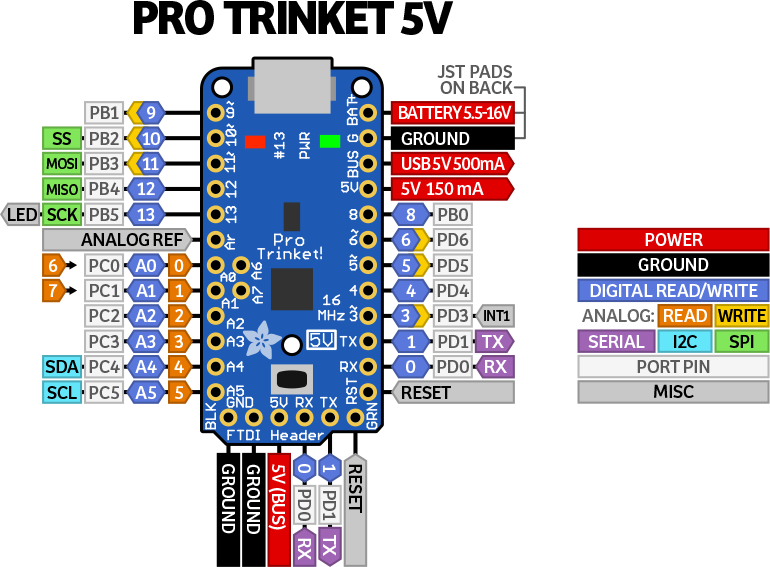
\includegraphics[width=0.5\textwidth]{adafruit_pro_trinket_5v.png}
	\caption[Adafruit Pro Trinket]{Adafruit Pro Trinket\protect\footnotemark}
	\label{fig:adafruit_pro_trinket}
	\source{\cite{adafruit2014protrinket}}
\end{figure}

\footnotetext{Der Adafruit Pro Trinket \SI{3.3}{\volt} ist zum Großteil pinkompatibel zu der \SI{5}{\volt} Variante. Nur der Pin \textit{BAT+} benötigte eine Batteriespannung von \SIrange{3.5}{16}{\volt} und der drei Reihen weiter unten liegende \SI{5}{\volt} Pin liefert nur \SI{3.3}{\volt}.}

Um eine Kommunikationsverbindung zwischem dem DWM1000 und dem Mikrocontroller herzustellen, müssen die Pins anhand der \tablename~\ref{tab:pin_assignment_between_dwm1k_and_pro_trinket} verbunden werden.

\begin{table}
	\centering
	\begin{tabular}{||c|c|c||} 
		\hline
		DWM1000 (Pin)&Pro Trinket (Pin)&Bedeutung\\\hline
		\hline
		SPICLK (20)&SCK (13)&SPI\\\hline
		SPIMISO (19)&MISO (12)&SPI\\\hline
		SPIMOSI (18)&MOSI (11)&SPI\\\hline
		SPICSn (17)&SS (10)&SPI\\\hline
		\hline
		IRQ (22)&INT1 (3)&Interrupt\\\hline
		\hline
		RSTn (3)&PB1 (9)&Hardware Reset\\\hline
	\end{tabular}
	\caption{Pinbelegung zwischen dem DWM1000 und Pro Trinket.}
	\label{tab:pin_assignment_between_dwm1k_and_pro_trinket}
\end{table}


\begin{comment}
% Lithium Ion Cylindrical Battery - 3.7v 2200mAh
% https://www.adafruit.com/product/1781
% Lithium Ion Polymer Battery - 3.7v 2500mAh
% https://www.adafruit.com/product/328
% Adafruit Pro Trinket LiPoly/LiIon Backpack
% https://learn.adafruit.com/adafruit-pro-trinket-lipoly-slash-liion-backpack?view=all
------------------------------------------------------------------------------------------
\end{comment}
\subsubsection{Energieversorgung}

Um den \gls{uwb}--Transceiver und den Pro Trinket mit Energie zu versorgen wird ein Lithiumionenakku mit einer Spannung von \SI{3.7}{\volt} und einer Kapazität von \SI{2200}{\mAh} verwendet. Die Verbindung zwischen den beiden wird über einen Lithiumionenakku Lade--Chip hergestellt. Diesen gibt es als fertiges Modul von Adafruit mit der Bezeichnung Pro Trinket LiPoly/LiIon Backpack.

Bevor jedoch dieses Modul eingesetz werden kann, müssen noch zwei Modifikationen durchgeführt werden. Zum einen kann die Energiequelle mittels eines Schalters vom Verbraucher getrennt werden. Per Standard sind jedoch diese zwei Pins mit einander verbunden und müssen mit einem schwarfen Messer unterbrochen werden, siehe \figurename~\ref{fig:pro_trinket_liion_backpack_top}. Zum anderen wird der Lithiumionakku nur mit einem Strom von \SI{100}{\mA} geladen. Bei einer Kapazität von \SI{2200}{\mAh} würde ein vollständiger Ladezyklus ca. \SI{22}{\hour} dauern. Um diese Zeit zu verkürzen, müssen die zwei Lötpads, siehe \figurename~\ref{fig:pro_trinket_liion_backpack_bottom}, miteinander verbunden werden. Danach wird der Lithiumionakku mit einem Strom von \SI{500}{\mA} geladen und demenstrechend verkürzt sich die Ladedauer auch auf ca. \SI{2.5}{\hour}.
%TODO: 2.5 Stunden? Häh? Wie wäre es mit 2 1/2, laut Duden korrekt.

\begin{figure}
	\centering
	\begin{subfigure}[t]{0.4\textwidth}
		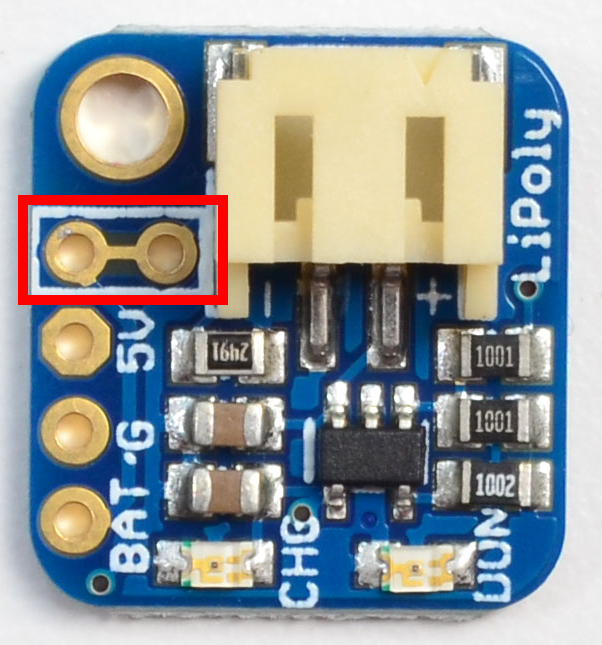
\includegraphics[width=\textwidth]{adafruit_lipoly_backpad_top_with_marker}
		\caption{Modifikation für den Schalter.}
		\label{fig:pro_trinket_liion_backpack_top}
	\end{subfigure}
	\qquad
	\begin{subfigure}[t]{0.4\textwidth}
		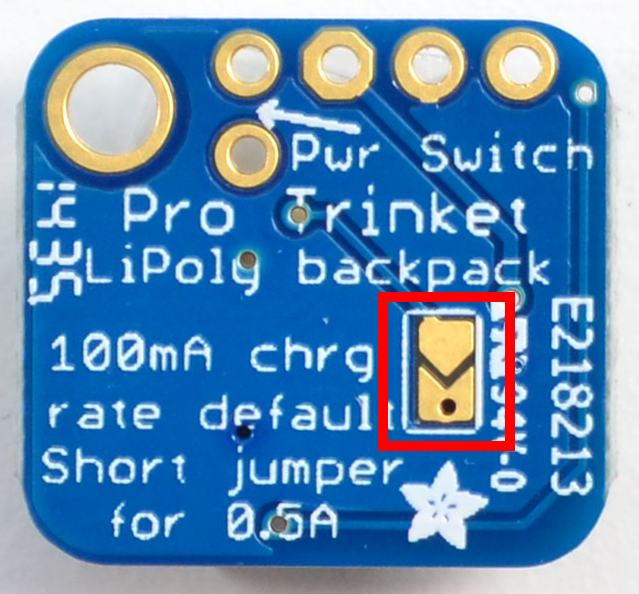
\includegraphics[width=\textwidth]{adafruit_lipoly_backpad_back_with_marker}
		\caption{Modifikation für einen höheren Ladestrom.}
		\label{fig:pro_trinket_liion_backpack_bottom}
	\end{subfigure}
	\caption{Adafruit Pro Trinket LiPoly/LiIon Backpack}
	\source{\cite{adafruit2014liionbackpack}}
	\label{fig:pro_trinket_liion_backpack}
\end{figure}
%TODO: URL ist zu lang und wird nicht umgebrochen.

Um eine Verbindung zwischem dem LiIon Backpack und dem Pro Trinket herzustellen, müssen die Pins anhand der \tablename~\ref{tab:pin_assignment_between_liion_backpack_and_pro_trinket} verbunden werden.

\begin{table}
	\centering
	\begin{tabular}{||c|c|c||} 
		\hline
		LiIon Backpack&Pro Trinket&Bedeutung\\\hline
		\hline
		BAT & BAT+ & Batteriespannung\\\hline
		5V & BUS & Ladespannung\\\hline
		G & GND & Masse\\\hline
		\hline
		SW1 & -- & Schalter\\\hline
		SW2 & -- & Schalter\\\hline
	\end{tabular}
	\caption{Pinbelegung zwischen dem LiIon Backpack und dem Pro Trinket.}
	\label{tab:pin_assignment_between_liion_backpack_and_pro_trinket}
\end{table}

Um den Lithium--Ion--Akku zu laden, bedarf es nicht mehr als den USB--Stecker des \textit{Pro Trinket} mit dem Computer oder einem USB--Ladegerät zu verbinden.


\begin{comment}
------------------------------------------------------------------------------------------
% Adafruit CP2104 Friend - USB to Serial Converter
% https://www.adafruit.com/product/3309
% https://www.silabs.com/documents/public/data-sheets/cp2104.pdf
% Universal Asynchronous Receiver Transmitter
% https://de.wikipedia.org/wiki/Universal_Asynchronous_Receiver_Transmitter
\end{comment}
\subsubsection{Datenaustausch}

% TODO: Computer? PC? Verarbeitungseinheit?
Der ATmega328/P verfügt nicht über einen eingebauten USB--Controller, daher ist ein direkter Datenaustausch zwischen dem Mikrocontroller und einem Computer nicht möglich. Jedoch verfügt der ATmega328/P über eine \gls{uart}--Schnittstelle, mit der Daten seriell über die Pins RX und TX übertragen und empfangen werden können. Mittels einem zusätzlichen Modul kann diesen Datenstrom aufgefangen und über die USB--Schnittstelle übertragen werden. Der CP2104 Friend von Adafruit erledigt genau diese Aufgabe. Angeschlossen wird er über den  \gls{ftdi}--Header, siehe \figurename~\ref{fig:adafruit_pro_trinket}. Dadurch ist es möglich die Module die einen Datenaustausch benötigen mit einem entsprechenden Modul auszurüsten.

% TODO: In jedem Abschnitt der gleiche Satz :$
Um eine Verbindung zwischem dem CP2104 Friend und dem Pro Trinket herzustellen, müssen die Pins anhand der \tablename~\ref{tab:pin_assignment_between_cp2104_and_pro_trinket} verbunden werden.

\begin{table}
	\centering
	\begin{tabular}{||c|c|c||} 
		\hline
		CP2104 Friend & Pro Trinket & Bedeutung\\\hline
		\hline
		GND & GND & Masse\\\hline
		CTS & GND & Masse\\\hline
		\hline
		5V & 5V & Versorgungsspannung\\\hline
		\hline
		TXD & RXD & Datenaustausch\\\hline
		RXD & TXD & Datenaustausch\\\hline
		\hline
		RTS & RTS & Reset\\\hline
	\end{tabular}
	\caption{Pinbelegung zwischen dem CP2104 Friend und dem Pro Trinket.}
	\label{tab:pin_assignment_between_cp2104_and_pro_trinket}
\end{table}


\begin{comment}
- Kosten für den Aufbau
------------------------------------------------------------------------------------------
\end{comment}
\subsubsection{Materialkosten pro \gls{uwbm}}

Die Materialkosten für einen \gls{tag} betragen jeweils \SI{45.15}{\euro} und für einen \gls{anchor} \SI{56.24}{\euro}. Der Unterschied ergibt sich dadurch, das z.B. für einen \gls{tag} keine Batterie benötigt wird, da dieser von der Energiequelle des Roboters gespeist wird.
Die detailierte Auflistung der Materialkosten können in der \tablename~\ref{tab:kosten_pro_modul} nachgeschlagen werden. Die Bauelemente die jeweils für einen \gls{tag} bzw. \gls{anchor} benötigt werden, sind in der dazugehörigen Spalte angekreuzt.

\begin{sidewaystable}
	\centering
	\begin{tabular}{||c|c|l|c|l|c|r||} 
		\hline
		\gls{tag} & \gls{anchor} & Anbieter & Artikelnummer & Komponente & Anzahl & Stückpreis\\\hline
		\hline
		\CheckedBox & \CheckedBox & Digi-Key & 1479-1002-1-ND & Decawave Limited DWM1000 & 1 & \SI{21.23}{\euro}\\\hline
		\CheckedBox & \CheckedBox & Digi-Key & 1528-1040-ND & Adafruit Pro Trinket \SI{3}{\volt} & 1 & \SI{8.25}{\euro}\\\hline
		\hline
		\CheckedBox & \CheckedBox & Conrad & 1417697-62 & Kohleschicht-Widerstand \SI{10}{\kilo\ohm} & 1 & \SI{0.06}{\euro}\\\hline
		\CheckedBox & \CheckedBox & Conrad & 1417644-62 & Kohleschicht-Widerstand \SI{180}{\ohm} & 4 & \SI{0.06}{\euro}\\\hline
		\CheckedBox & \CheckedBox & Conrad & 180134-62 & LED Grün & 2 & \SI{0.25}{\euro}\\\hline
		\CheckedBox & \CheckedBox & Conrad & 184756-62 & LED Rot & 2 & \SI{0.34}{\euro}\\\hline
		\Square & \CheckedBox & Conrad & 251007-62 & Emmerich LiIon Akku ICR-18650 NH-SP& 1 & \SI{9.99}{\euro}\\\hline
		\hline
		\Square & \CheckedBox & EXP-Tech & EXP-R15-577 & Adafruit Pro Trinket LiPoly/LiIon Backpack & 1 & \SI{5.55}{\euro}\\\hline
		\CheckedBox & \Square & EXP-Tech & EXP-R15-1157 & Adafruit CP2104 Friend & 1 & \SI{6.45}{\euro}\\\hline
		\Square & \CheckedBox & EXP-Tech & EXP-R15-419 & Breadboard-friendly SPDT Slide Switch & 1 & \SI{1.20}{\euro}\\\hline
		\Square & \CheckedBox & EXP-Tech & EXP-R15-1074 & JST 2-Pin Cable & 1 & \SI{0.80}{\euro}\\\hline
		\hline
		\CheckedBox & \CheckedBox & AISLER & -- & \acrlong{pcb} & 1 & \SI{7.74}{\euro}\\\hline
		\hline
		\multicolumn{6}{|r|}{Gesamtpreis für einen \gls{tag}:} & \SI{45.15}{\euro}\\\hline
		\multicolumn{6}{|r|}{Gesamtpreis für einen \gls{anchor}:} & \SI{56.24}{\euro}\\\hline
	\end{tabular}
	\caption{Materialkosten pro \gls{tag} bzw. \gls{anchor}.}
	\label{tab:kosten_pro_modul}
\end{sidewaystable}


\begin{comment}
- Schaltplan-Skizze
	- Besonderheiten (NetLabels)
	- SVG/PNG/PDF-Export
	- Gruppierung nach Funktionsgruppen
------------------------------------------------------------------------------------------
\end{comment}
\subsubsection{Schaltplan} \label{subsec:schaltplan_uwb_modul}

Eine Übersicht der besprochenen Bauelemente, gruppiert nach Funktionsgruppen, können dem Schaltplan in \figurename~\ref{fig:schaltplan_uwb_modul} entnommen werden.

\begin{figure}
	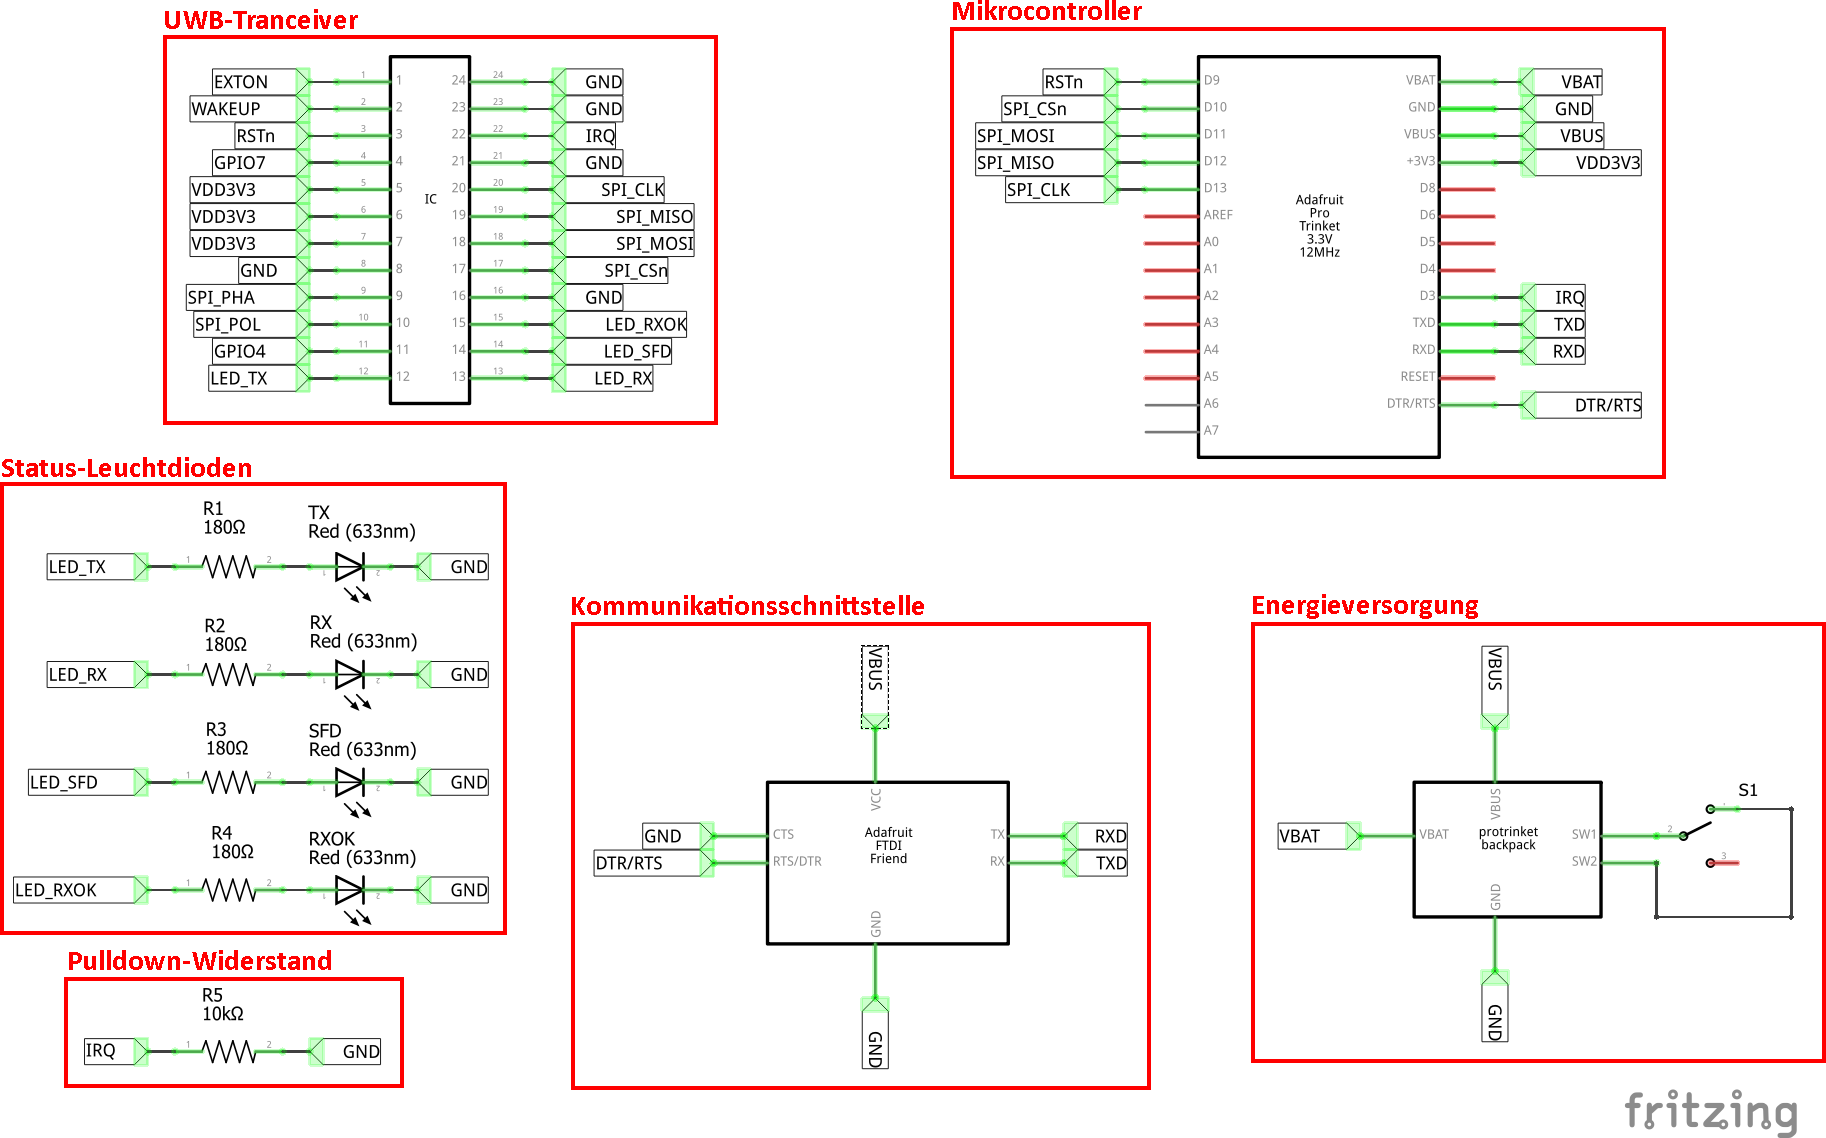
\includegraphics[width=\textwidth]{Trinket_And_DWM1000_v3_schem}
	\caption{Schaltplan des \gls{uwb}--Moduls.}
	\label{fig:schaltplan_uwb_modul}
\end{figure}


\begin{comment}
------------------------------------------------------------------------------------------
- 1. Prototyp Aufbau auf einem Breadboard
	- UWB-Adapter von ...?
	- SMD Löttechnik
	- Funktionstest
	- Skript als Anhang
- 2. Prototyp Aufbau auf einem Lochstreifen
	- Kommunikations- und Entfernungsmessungstest
\end{comment}
\subsection{Prototypen}

Anhand eines vorläufigen Schaltplans wurden zwei Prototypen erstellt, siehe \figurename~\ref{fig:prototypen_der_uwb_module}.

Der erste Prototyp wurde auf einer Steckplatine realisiert, siehe \figurename~\ref{fig:prototyp_eins_uwb_modul}. Die elektrische Verbindung zu dem DWM1000 \gls{ic} wurde dabei über eine Freiluftverdrahtung mit einem steckplatinenfähigen Adapter umgesetzt. Der erste Verbindungsaufbau wurde dabei mit dem Beispielprogramm \textit{BasicConnectivityTest} aus dem GitHub--Projekt \cite{Trojer2015} durchgeführt. Hierbei ist zu beachten das der \textit{PIN\_IRQ} bei dem \textit{Pro Trinket} nicht auf Pin 2 sondern auf Pin 3 liegt.

Während dem Aufbau des ersten Prototypen wurde ein \gls{pcb}--Adapterboard, siehe \figurename~\ref{fig:pcb_dwm1000_adapterboard_top}, für den DWM1000 bestellt. Dieses \gls{pcb}--Adapterboard wurde ebenfalls dem GitHub--Projekt \cite{Trojer2015} entnommen. Mit diesem wurde dann ein zweiter Prototyp aufgebaut, siehe \figurename~\ref{fig:prototyp_zwei_uwb_modul}, der zusätzlich ohne eine externe Energieversorgung betrieben werden konnte. Mittels der beiden Prototypen war ein erster Nachrichtenaustausch bzw. eine erste Entfernungsmessung möglich. Der Nachrichtenaustauch wurden mit den Beispielprogrammen \textit{BasicReceiver} und \textit{BasicSender} erprobt, die Entfernungsmessung mit \textit{RangingAnchor} und \textit{RangingTag}.

\begin{figure}
	\begin{subfigure}[t]{0.4\textwidth}
		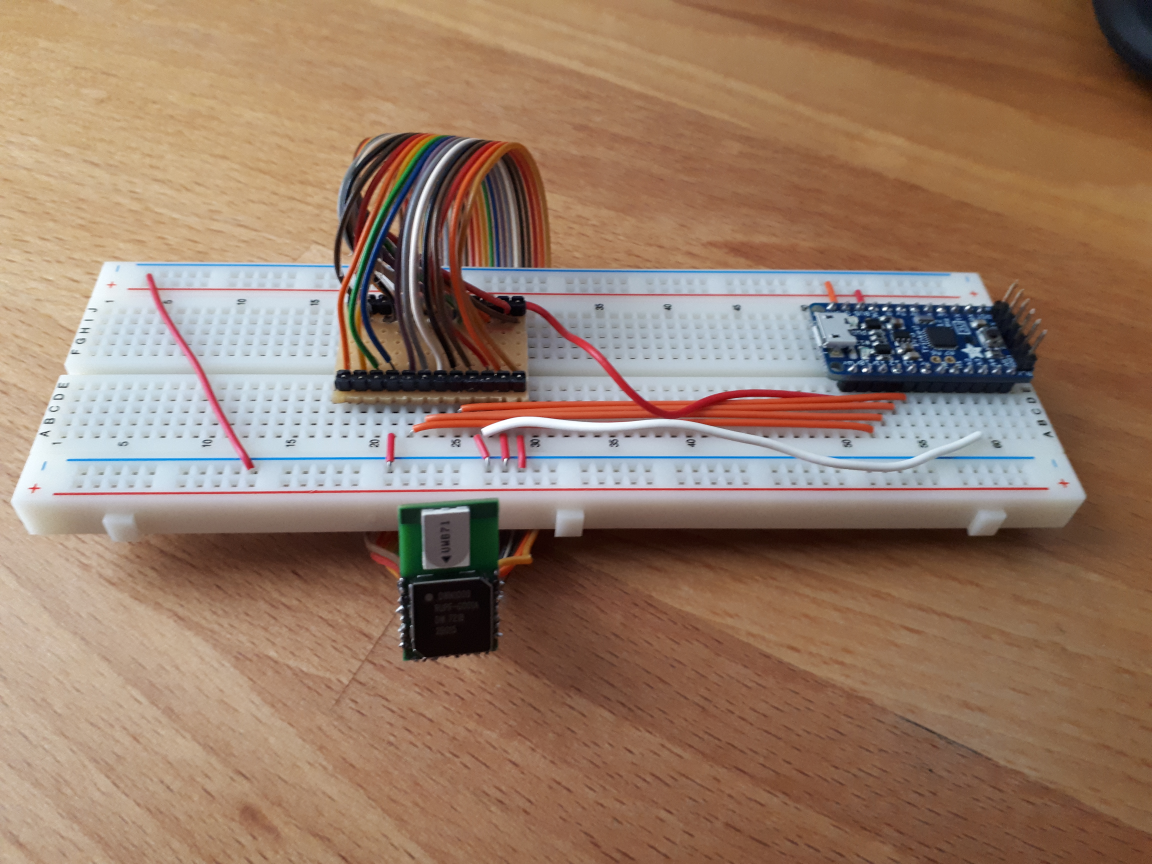
\includegraphics[width=\textwidth]{prototyp_eins_uwb_modul}
		\caption{Erster Prototyp auf einer Steckplatine.}
		\label{fig:prototyp_eins_uwb_modul}
	\end{subfigure}
	\hfill
	\begin{subfigure}[t]{0.4\textwidth}
		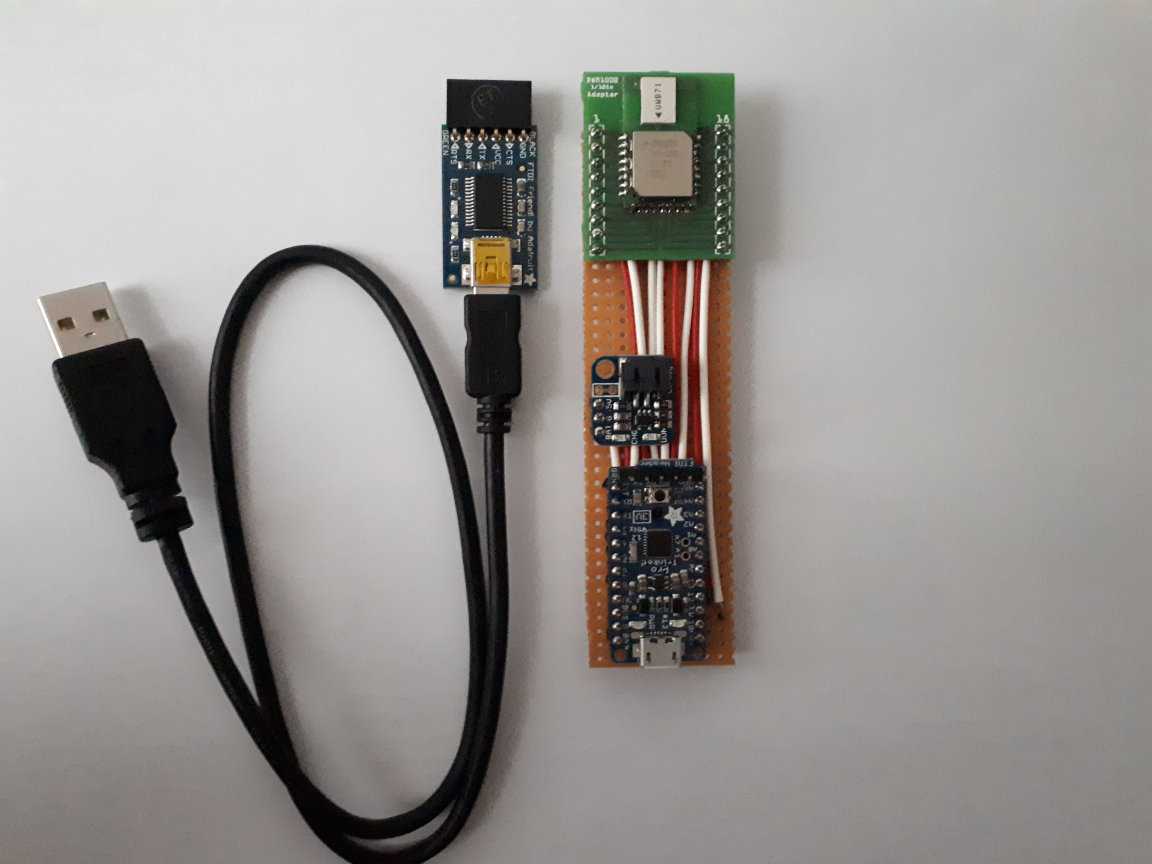
\includegraphics[width=\textwidth]{prototyp_zwei_uwb_modul}
		\caption{Zweiter Prototyp auf einem Lochstreifen.}
		\label{fig:prototyp_zwei_uwb_modul}
	\end{subfigure}
	\caption{Die ersten zwei Prototypen der \glspl{uwbm}.}
	\label{fig:prototypen_der_uwb_module}
\end{figure}

\begin{figure}
%\begin{wrapfigure}{r}{0.3\textwidth}
  \centering
  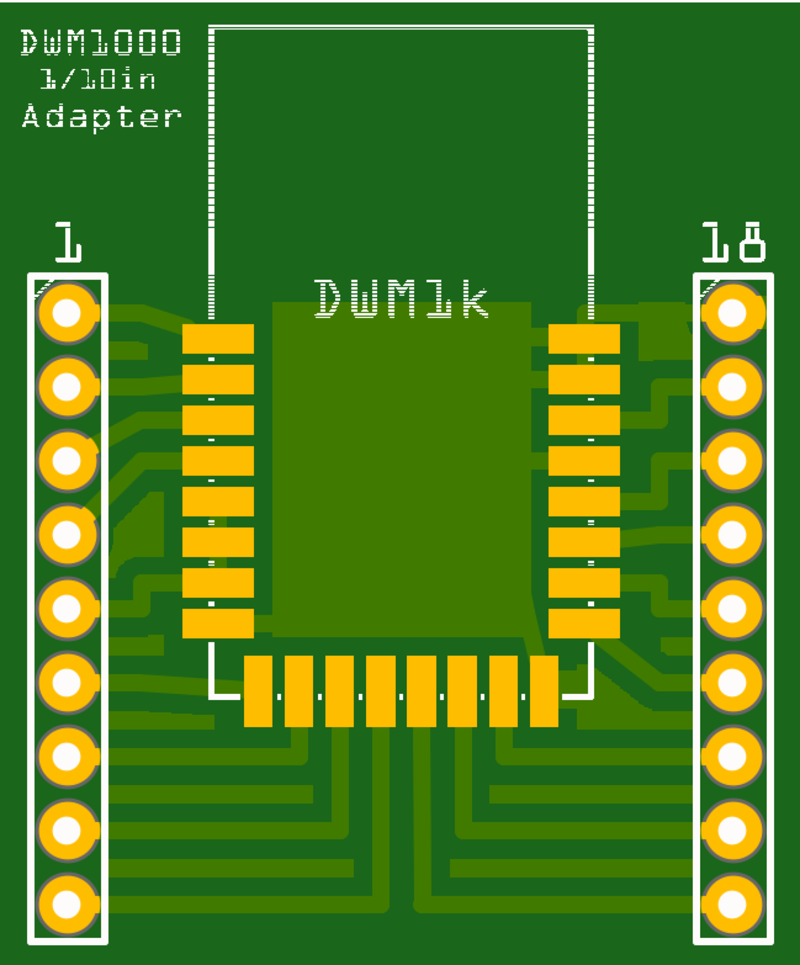
\includegraphics[width=0.28\textwidth]{pcb_dwm1000_adapterboard_top}
  \caption{\gls{pcb}--Adapterboard für den DWM1000.}
  \label{fig:pcb_dwm1000_adapterboard_top}
%\end{wrapfigure}
\end{figure}


\begin{comment}
------------------------------------------------------------------------------------------
+ Der initiale Aufbau erfolgt zu Evaluationszwecken auf einem Steckboard und zusätzlich auf einer separaten Lochstreifenplatine um das Zusammenspiel zweier UWB--Module zu testen. Nach dem erfolgreichen Systemtest wird aus dem erstellten Schaltplan, ein PCB--Layout erstellt, mehrere PCB--Boards bestellt und nach der Lieferung zusammengebaut und noch mal getestet.
+ Antenne
+ Aufrecht stehend
+ Batterie auf der Rückseite bietet stabilität
	+ Flachere Akkus können auch verwendet werden
+ Ansteckbares FTDI
+ Preis pro Platinengröße
- Footprint of DWM1000
+ AutoRoute
- TODO: Ground Fill with Copper
- Wikipedia: In der Antennentechnik (Satellitenfunk) bezeichnet der Azimutwinkel die horizontale Ausrichtung einer Antenne, im Gegensatz zur Elevation, die den vertikalen Winkel zwischen Horizont und Antennenrichtung angibt.
\end{comment}
\subsection{Platinendesign}

Nachdem die Korrektheit des Schaltplans durch die Prototypen bestätigt wurde, kann nun das Layout für die entgültigen \gls{pcb}--Platinen erstellt werden. Sowohl der Schaltplan als auch das Platinen--Layout werden mit dem Programm \textit{fritzing}\cite{fritzing} erstellt. Jedes im Schaltplan verwendete elektrische Bauelement besitzt einen \gls{footprint}, der die Größe des Bauelementes und seine elektrischen Anschlüsse auf der Leiterplatte festlegt, siehe \figurename~\ref{fig:breadboard_schematic_pcb}. Anhand des \glspl{footprint} muss nun jedes Bauteil so plaziert werden, das es idealerweise möglichst wenig Platz auf der Leiterplatte verschwendet wird. Den je kleiner die Leiterplatte ist, desto günstiger in der Herstellung.

\begin{figure}
	\begin{subfigure}[t]{0.3\textwidth}
		\centering
		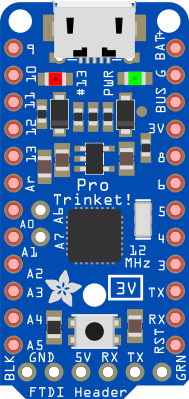
\includegraphics[width=0.5\textwidth]{pro_trinket_breadboard}
		\caption{Reales Bauelement}
		\label{fig:pro_trinket_breadboard}
	\end{subfigure}
	\quad
	\begin{subfigure}[t]{0.3\textwidth}
		\centering
		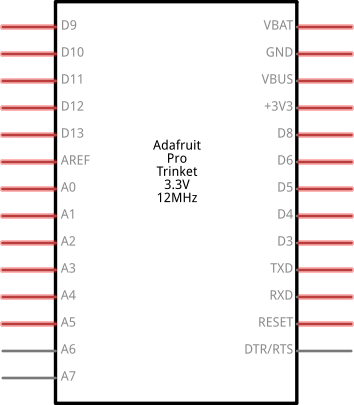
\includegraphics[width=\textwidth]{pro_trinket_schematic}
		\caption{Bauelement im Schaltplan}
		\label{fig:pro_trinket_schematic}
	\end{subfigure}
	\quad
	\begin{subfigure}[t]{0.3\textwidth}
		\centering
		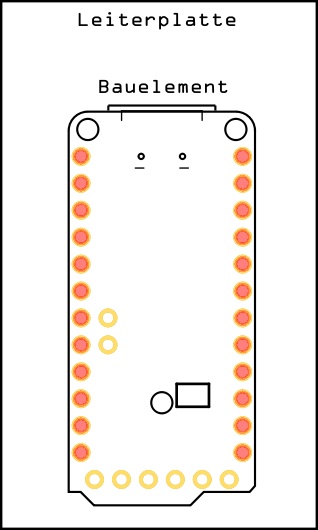
\includegraphics[width=\textwidth]{pro_trinket_pcb}
		\caption{Bauelement mit seinem \gls{footprint} auf einer Leiterplatte.}
		\label{fig:pro_trinket_pcb}
	\end{subfigure}
	\caption{Designstufen eines elektrischen Bauelementes.}
	\label{fig:breadboard_schematic_pcb}
\end{figure}

Die Leiterplatte besitzt eine rechteckige Form, mit den Maßen \SI{43 x 75}{\mm}. Am höchsten Punkt der Leiterplatte befindet sich die Antenne des \gls{uwbt}, dadurch wird gewährleistet das die Antenne in horizontaler Richtung ein gleichmäßiges Abstrahlmuster aufweist, siehe \figurename~\ref{fig:dwm1000_antenna_radiation_pattern}. Desweiteren empfehlen die \textit{Application Board Layout Guidelines} das unterhalb der Antenne sich keine Metall oder andere nicht RF transparente Materialien befinden und ein freier horizontaler Abstand von mindestens \SI{10}{\mm} eingehalten wird, siehe \figurename~\ref{fig:dwm1000_application_board_keep_out_areas}.

Links neben dem \gls{uwbt} befinden sich gut sichtbar die Status-Leuchtdioden. Unterhalb der Status-Leuchtdioden befindet sich der Ladeschaltkreis für die Lithium-Ion Batterie sowie der Ein--Aus--Schalter. Auf der Rückseite der Leiterplatte wird die Batterie befestigt. Dadurch ist ein aufrechter Stand des \gls{uwbm} möglich. Die Leiterplatte ist mit \SI{75}{\mm} ca. \SI{10}{\mm} größer als die Batterie, sodass es zu keiner Beeinträchtigung der Antenne kommen sollte.

Im unteren rechten Bereich der Leiterplatte befindet sich der \textit{Pro Trinket}, also die Verarbeitungseinheit. Direkt daneben auf der linken Seite ist das optionale Datenübertragungsmodul vorgesehen. Da der \gls{tag} auf dem Roboter in einer erhöhten Position befestigt wird, zeigt der USB--Stecker für das Datenübertragunsmodul in eine ideal Richtung.

Nachdem jedes elektrische Bauelement auf der Leiterplatte positioniert wurde, muss noch die Verdrahtung der einzelnen Bauelemente erfolgen. Sehr bequem erfolgt die Verdrahtung über die \textit{Autoroute}--Funktion. Hierbei errechnet ein Algorithmus, welchen Weg die Leiterbahnen nehmen sollen um alle notwendigen Pins miteinander zu verbindungen ohne das sich ihre Wege überschneiden. Das fertige Layout der Leiterplatte ist in \figurename~\ref{fig:pcb_uwb_modul_board_top} abgebildet. In der \figurename~\ref{fig:uwb_modul} ist ein fertig aufgebautes \gls{uwbm} abgebildet.

\begin{figure}
	\centering
	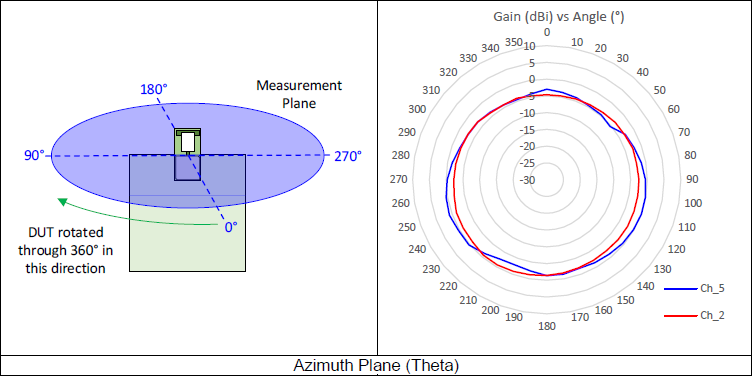
\includegraphics[width=\textwidth]{dwm1000_antenna_radiation_pattern}
	\caption{Das Antennenabstrahlmuster in horizontaler Richtung.}
	\label{fig:dwm1000_antenna_radiation_pattern}
	\source{\cite{decawave2016dwm1kdatasheet}}
\end{figure}
	
\begin{figure}
	\centering
	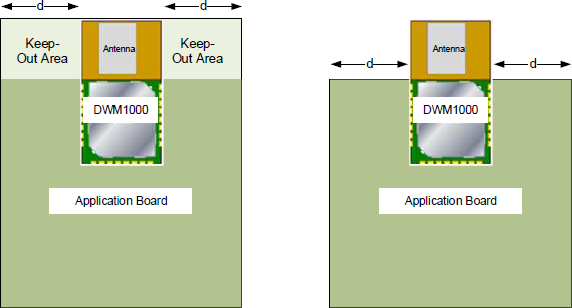
\includegraphics[width=\textwidth]{dwm1000_application_board_keep_out_areas}
	\caption{Antennenfreiräume}
	\label{fig:dwm1000_application_board_keep_out_areas}
	\source{\cite{decawave2016dwm1kdatasheet}}
\end{figure}

%\begin{figure}
%	\centering
%	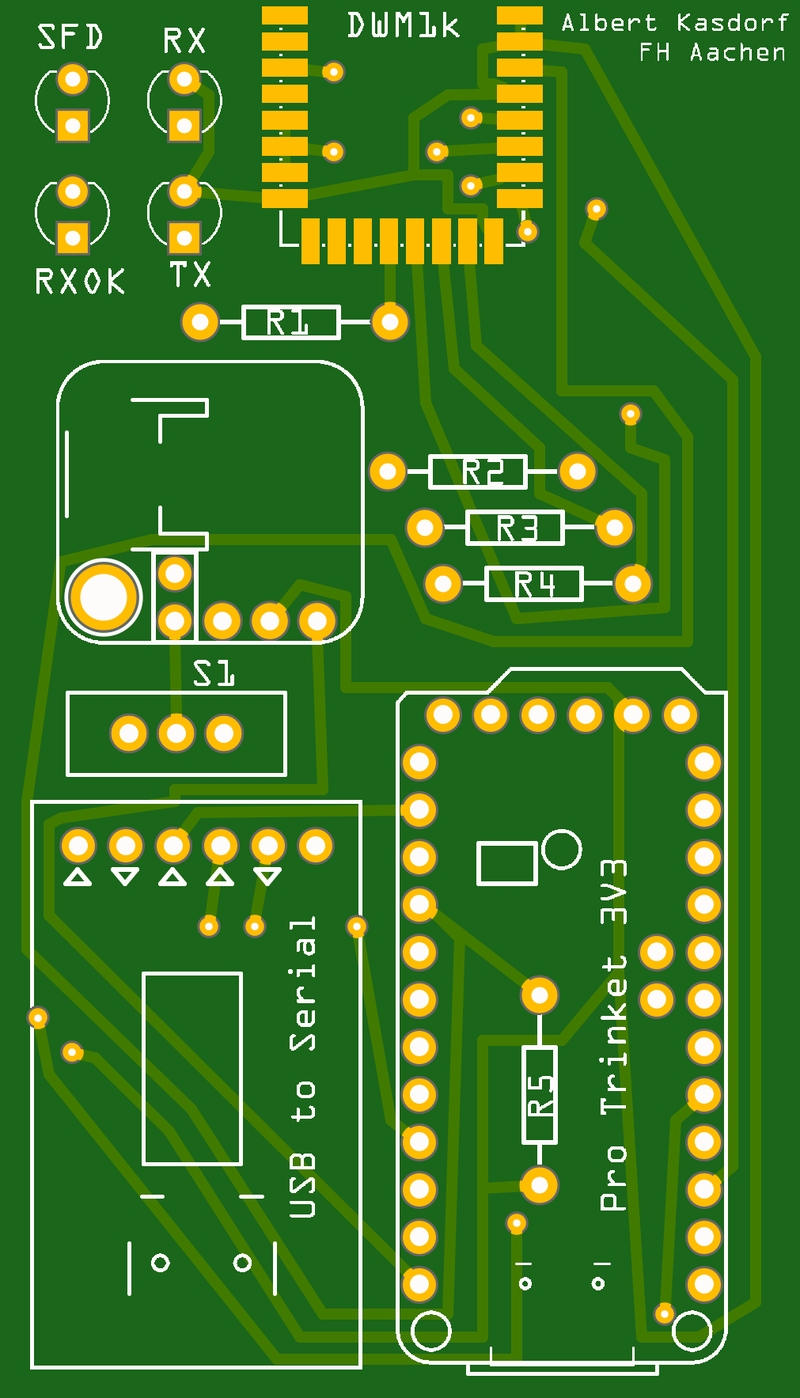
\includegraphics[width=0.25\textwidth]{pcb_uwb_modul_board_top}
%	\caption{Das fertige Leiterplatten Layout.}
%	\label{fig:pcb_uwb_modul_board_top}
%\end{figure}
%
%\begin{figure}
%	\centering
%	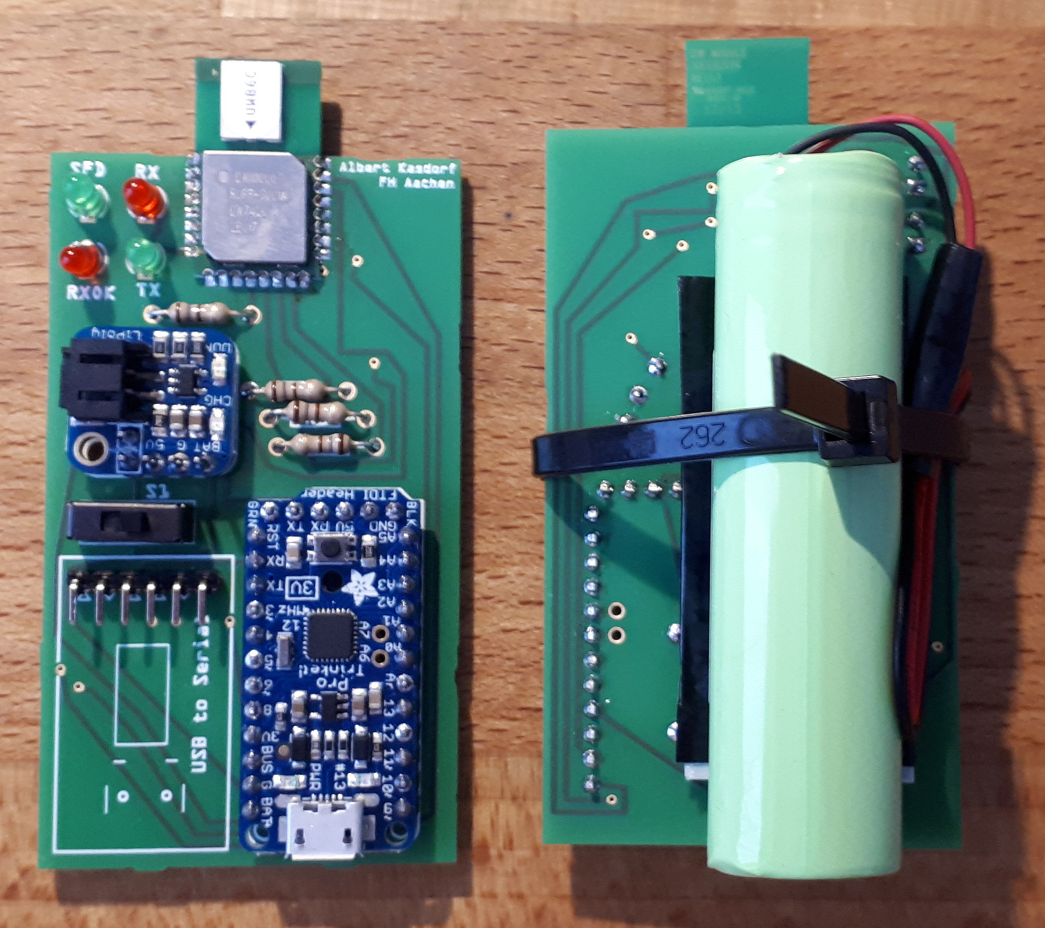
\includegraphics[width=0.5\textwidth]{uwb_modul}
%	\caption{Vorder- und Rückansicht eines \gls{uwbm}.}
%	\label{fig:uwb_modul}
%\end{figure}

\begin{figure}
	%\centering
	\begin{subfigure}[t]{0.3\textwidth}
		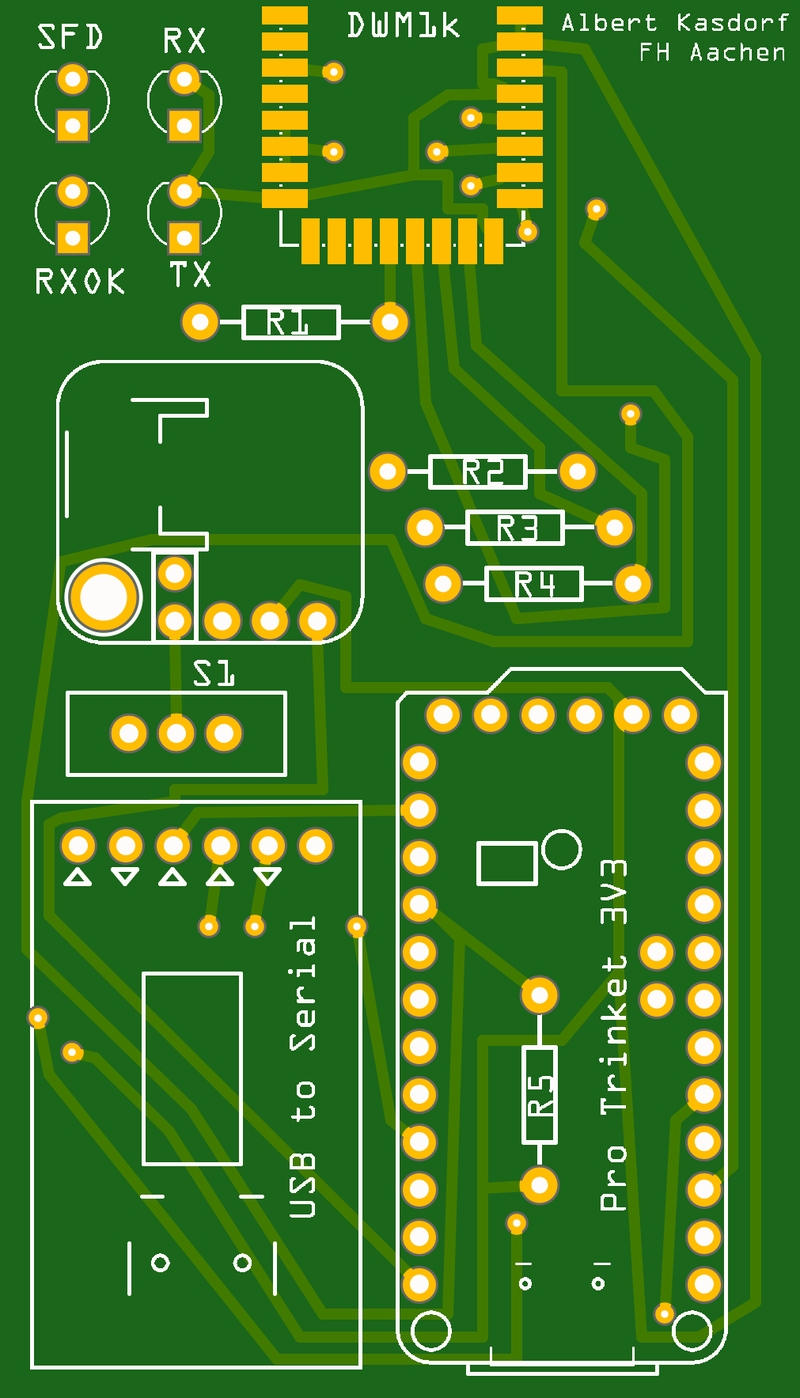
\includegraphics[width=\textwidth]{pcb_uwb_modul_board_top}
		\caption{Das fertige Leiterplatten Layout.}
		\label{fig:pcb_uwb_modul_board_top}
	\end{subfigure}
	\hfill
	\begin{subfigure}[t]{0.6\textwidth}
		\centering
		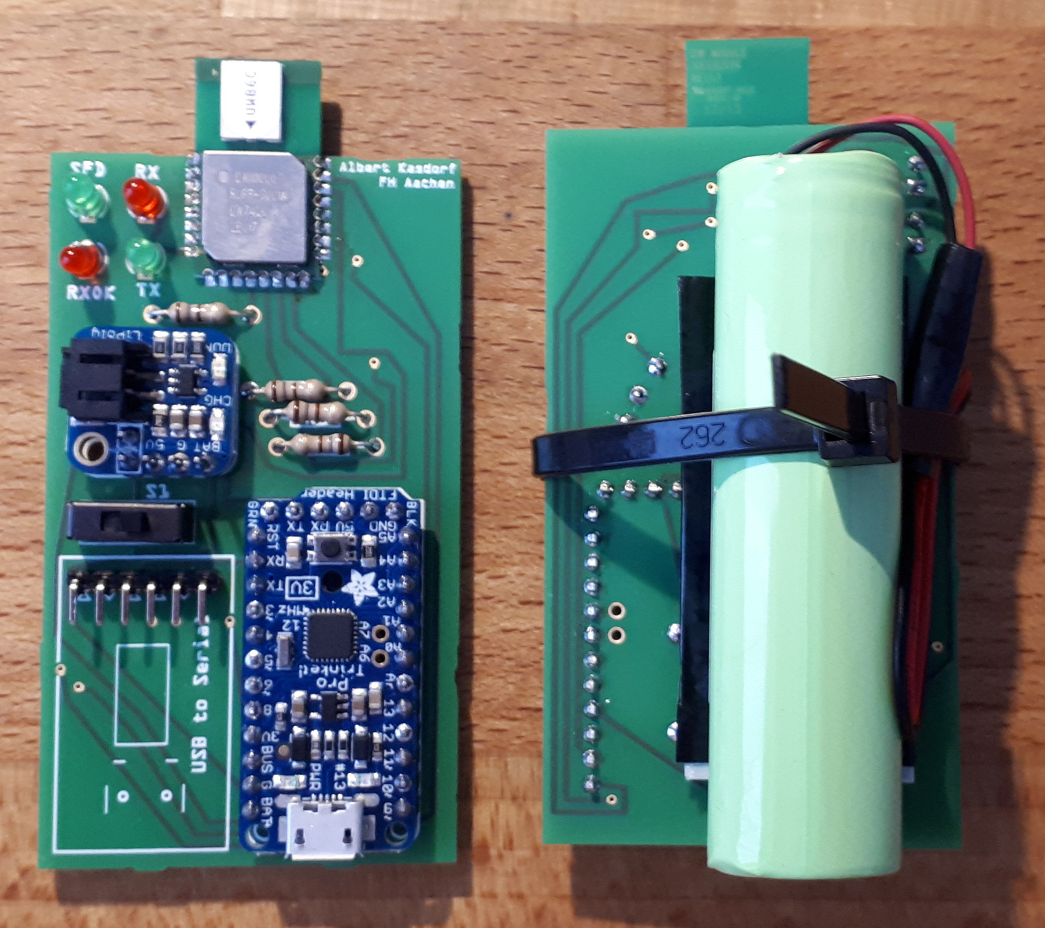
\includegraphics[width=\textwidth]{uwb_modul}
		\caption{Vorder- und Rückansicht eines \gls{uwbm}.}
		\label{fig:uwb_modul}
	\end{subfigure}
	\caption{Fertige \glspl{uwbm}.}
	\label{fig:fertige_uwb_module}
\end{figure}


\begin{comment}
------------------------------------------------------------------------------------------
- Woher kommt die Steuersoftware und wer ist für diese Zustandig?
	- Aktive Entwicklung wurde eingestellt
	- Was kann ich mit dieser Software machen?
\end{comment}
\subsection{Steuersoftware}

Als Basis für die Steuersoftware wurde das GitHub--Projekt \cite{Trojer2015} verwendet. Neben einer stabilen Basis für die Kommunikation mit dem \textit{DWM1000}, existiert eine Implementierung des \Gls{twr}--Verfahrens von \textit{DecaWave}. Die aktive Entwicklung ist mittlerweile eingestellt, es werden jedoch weiterhin \textit{Pull--Requests\footnotemark} für Fehlerkorrekturen und neue Funktionalitäten angenommen.

% https://blog.seibert-media.net/blog/2014/05/12/git-workflows-der-pull-request-workflow-teil-1/
\footnotetext{Ein Pull--Request dient dazu, eine Weiterentwicklung oder Fehlerkorrektur mit anderen Entwicklern zu disktuieren und dann auf einfach Weise in den Hauptentwicklungszweig zu integrieren.}


\begin{comment}
------------------------------------------------------------------------------------------
- Klassendiagramme der wichtigsten Elemente
	- Auswelchen wichtigen Elementen besteht diese Bibliothek?
	- DW1000
	- DW1000Time
	- DW1000Device
	- DW1000Ranging
- Die Steuersoftware besteht aus den Klassen \textit{DW1000}, \textit{DW1000Time}, \textit{DW1000Ranging}, \textit{DW1000Device} die im folgenden Beschrieben werden.
\end{comment}
\subsubsection{Klassenübersicht}

Die Klasse \textit{DW1000} enthält alle Basisfunktionalität um mit dem \textit{DWM1000} arbeiten zukönnen. Dazu gehören die Kommunikation über den \Gls{spi}--Bus, das Lesen und Schreiben der Konfiguration und das Erstellen und Empfangen von Nachrichten. Über einen Low--Level Zugriff ist es zusätzlich möglich auf Funktionalitäten des \textit{DW1000} zuzugreifen die in dem ursprunglichen Klassendesign nicht vorgesehen waren.

Zeitstempel spielen beim Nachrichtenaustausch und bei der Entfernungsmessung eine zentrale Rolle. Jedoch werden die Zeitstempel als \SI{40}{\bit} Zahl gespeichert. Um die Verwendung zu erleichtern und Fehlerquellen auszuschließen wurde die Hilfsklasse \textit{DW1000Time} bereitgestellt.

Über die Klasse \textit{DW1000Ranging} ist eine Implementierung des \Gls{twr}--Verfahrens von \textit{DecaWave} verfügbar. Mittels drei Rückruffunktionen (engl. Callback function) teilt die Klasse dem Anwender mit, welche Entfernungen gemessen wurde und ob neue Quellen für Entfernungsmessungen hinzugekommen oder verschwunden sind. Jede Quelle für eine Entfernungsmessung wird mit der Klasse \textit{DW1000Device} modelliert. Neben der gemessenen Entfernung beinhaltet die Klasse auch eine eindeutige Identifikationsnummer. 


\begin{comment}
------------------------------------------------------------------------------------------
- Basisscript
	- Wie sieht ein ganz triviales Beispiel aus?
	- Wie ist der Programmablauf des Beispiels?
	- Für das DW1000Ranging
	- Wie kann man Daten austauschen? JSON
- Datenaustausch zwischen Host und µC
- ArduinoJson Assistant
	- https://arduinojson.org/assistant/
\end{comment}
\subsubsection{Datenaustausch}

Der erste Bereich des Datenaustausches findet zwischen den \Glspl{uwbm}n statt. Hierfür wird mindestens ein \Gls{anchor} und \Gls{tag} benötigt. In der \lstlistingname~\ref{lst:uwb_modul_as_anchor} ist der Quellcode eines \Gls{anchor} abgebildet.
Über die ersten zwei Zeile wird die \textit{\Gls{spi}--} und \textit{DW1000Ranging}--Bibliothek in das Programm eingebunden.
Um eine Kommunikation mit dem \textit{DWM1000} aufzubauen muss der Methode \textit{initCommunication} die Belegung des \textit{Reset--}, \textit{\Gls{ss}--} und \textit{\Gls{irq}--Pin} übergeben werden.
Nach dem Aufruf der Methode \textit{startAsAnchor} fungiert das \Gls{uwbm} als \Gls{anchor}. Die notwendigen Parameter sind dabei die eindeutige Adresse, der Messmodus und ob eine zufällige Geräteadresse generiert werden soll. Wenn der letzte Parameter \textit{false} ist, werden aus den ersten zwei Bytes der eindeutigen Adresse, die Geräteadresse gebildet. Der zyklische Aufruf der Methode \textit{loop} sorgt für die Nachrichtenverarbeitung des \Gls{uwbm}s.

\begin{lstlisting}[
	frame=shadowbox,
	breaklines=true,
	caption={Quellcode für ein \Gls{uwbm} das als \Gls{anchor} konfiguriert ist.},
	captionpos=b,
	label={lst:uwb_modul_as_anchor},
	language=C++,
	columns=fullflexible,
	numbers=none,
	float,
]
#include <SPI.h>
#include <DW1000Ranging.h>

void setup() {
  Serial.begin(115200);

  DW1000Ranging.initCommunication(9, SS, 3);
  
  DW1000Ranging.startAsAnchor("B1:00:00:00:B1:6B:00:B5",
    DW1000.MODE_LONGDATA_RANGE_ACCURACY, false);
}

void loop() { DW1000Ranging.loop(); }
\end{lstlisting}

Das Gegenstück zum \Gls{anchor} ist in der \lstlistingname~\ref{lst:uwb_modul_as_tag} abgebildet. Jede gemessene Entfernung zwischen dem \Gls{tag} und einem \Gls{anchor} soll per \Gls{usb} an den Computer übertragen werden. Der Datenaustausch erfolgt dabei im \Gls{json}--Format, daher wird die Bibliothek \textit{ArduinoJson} benötigt.
Da dieses \Gls{uwbm} als \Gls{tag} fungieren soll, muss anstatt \textit{startAsAnchor} die Methode \textit{startAsTag} aufgerufen werden. Die Bedeutung der Parameter zwischen den beiden Methoden bleibt identisch.
Neu ist der Aufruf der Methode \textit{attachNewRange}, \textit{attachNewDevice} und \textit{attachInactiveDevice}. Jeder der Methoden wird die Adresse einer Rückruffunktion übergeben. Diese Funktionen werden immer dann aufgerufen, wenn eine neue Entfernungen gemessen wurde und wenn eine neue Quellen für die Entfernungsmessungen hinzugekommen oder verschwunden ist.
Alle Rückruffunktionen rufen ihrerseit die Funktion \textit{transmitDATA} auf. In dieser wird mittels der Klasse \textit{StaticJsonBuffer} ein \textit{JsonObject} erstellt, mit Daten im Schlüssel--Wert--Format (engl. Key--Value) belegt und dann mittels der Methode \textit{printTo(Serial)} über die \Gls{usb}--Schnittstelle an den Computer versendet. Das Format der Daten ist in der \lstlistingname~\ref{lst:data_in_json_format} abgebildet.

\begin{lstlisting}[
	frame=shadowbox,
	breaklines=true,
	caption={Quellcode für ein \Gls{uwbm} das als \Gls{tag} konfiguriert ist.},
	captionpos=b,
	label={lst:uwb_modul_as_tag},
	language=C++,
	columns=fullflexible,
	numbers=none,
	float,
]
#include <SPI.h>
#include <DW1000Ranging.h>
#include <ArduinoJson.h>

enum class Events : byte {
  NEW_RANGE=0, NEW_DEVICE=1, INACTIVE_DEVICE=2
};

void setup() {
  Serial.begin(115200);
  
  DW1000Ranging.initCommunication(9, SS, 3);
  DW1000Ranging.attachNewRange(newRange);
  DW1000Ranging.attachNewDevice(newDevice);
  DW1000Ranging.attachInactiveDevice(inactiveDevice);

  DW1000Ranging.startAsTag("A0:00:00:00:B1:6B:00:B5",
    DW1000.MODE_LONGDATA_RANGE_ACCURACY, false);
}

void loop() {
  DW1000Ranging.loop();
}

void newRange() {
  transmitDATA(Events::NEW_RANGE, DW1000Ranging.getDistantDevice());
}

void newDevice(DW1000Device* device) {
  transmitDATA(Events::NEW_DEVICE, device);
}

void inactiveDevice(DW1000Device* device) {
  transmitDATA(Events::INACTIVE_DEVICE, device);
}

void transmitDATA(const Events event, const DW1000Device* device) {
  StaticJsonBuffer<200> jsonBuffer;
  JsonObject& root = jsonBuffer.createObject();

  root["type"] = static_cast<byte>(event);
  root["aa"] = device->getShortAddress();
  root["r"] = (event==Events::NEW_RANGE) ? device->getRange() : 0.0f;
  
  root.printTo(Serial);
  Serial.println();
}
\end{lstlisting}

\begin{lstlisting}[
	frame=shadowbox,
	breaklines=true,
	caption={Datenzeile im \Gls{json}--Format beim Austausch zwischen \Gls{uwbm} und Computer.},
	captionpos=b,
	label={lst:data_in_json_format},
	columns=fullflexible,
	numbers=none,
	float,
]
{"type": 0, "aa": 160, "r": 1.01}
\end{lstlisting}

Nach dem die Daten an den Computer gesendet wurde, müssen diese entgegengenommen und in das \Gls{ros}--System eingespeist werden. Dies geschieht über die \lstlistingname~\ref{lst:json_to_ros}.
Zuerst wird das \Gls{ros}--System über \textit{rospy.init\_node} initalisiert. Um Nachrichten versendet zu können, wird zusätzlich ein \textit{Publisher} benötigt. Dieser wird über den Aufruf von \textit{rospy.Publisher} erstellt. Die Verbindung zu dem \Gls{uwbm} wird über den Aufruf \textit{serial.Serial} hergestellt.
Mittels der \Gls{ros}--Nachricht \textit{ObservationRangeBeacon} wird die Sensor--Charakteristik des \Gls{uwbm}s beschrieben. Hierzu gehören die minimal und maximal messbare Entfernung, das Sensorrauschen, eine oder mehrere Entfernungsmessungen und einige \Gls{ros} spezifische Angaben wie z.B. das Koordinatensystem in dem sich das \Gls{uwbm} befindet.
Danach werden solange Daten von dem \Gls{uwbm} gelesen bis der \Gls{ros}--Knoten beendet wird. Jeder gelesen Datensatz wird mittels der Methode \textit{json.loads(line)} untersucht, in ein \Gls{json}--Objekt konvertiert, und im Fehlerfall übersprungen. Gültige Entfernungsdaten werden in den Attributen \textit{range} und \textit{id} des Feldes \textit{orb.sensed\_data} gespeichert.
Der Aufruf \textit{pub.publish(orb)} übergibt die zuvor erstellte Nachricht an das \Gls{ros}--System.

\begin{lstlisting}[
	frame=shadowbox,
	breaklines=true,
	caption={JSON to ROS OberservationRangeBeacon},
	captionpos=b,
	label={lst:json_to_ros},
	language=Python,
	columns=fullflexible,
	numbers=none,
	float,
]
import json
import rospy
import serial

from mrpt_msgs.msg import ObservationRangeBeacon
from mrpt_msgs.msg import SingleRangeBeaconObservation

def main():
  rospy.init_node('beacon_publisher')
  pub = rospy.Publisher('/beacon', ObservationRangeBeacon, queue_size=10)
  ser = serial.Serial('/dev/CP2104_Friend', 115200, timeout=2)

  orb = ObservationRangeBeacon()
  orb.header.frame_id = 'uwb_reciever_link'
  orb.min_sensor_distance = 0.0
  orb.max_sensor_distance = 120.0
  orb.sensor_std_range = 0.1
  orb.sensed_data.append(SingleRangeBeaconObservation())

  while not rospy.is_shutdown():
    line = ser.readline()
    try:
      obj = json.loads(line)
    except ValueError:
      continue

    orb.header.stamp = rospy.Time.now()
    orb.header.seq = orb.header.seq + 1
    orb.sensed_data[0].range = obj["r"]
    orb.sensed_data[0].id = obj["aa"]

    pub.publish(orb)
\end{lstlisting}

Der vollständige Quellcode mit Kommentaren und Fehlerbehandlung kann in dem GitHub--Projekt \cite{kasdorf2017roslamwithuwb} eingesehen werden.


\begin{comment}
------------------------------------------------------------------------------------------
- Kalibierung nach DecaWave
	- FlowCharts erklären
	- Ergebnisse auswerten
- Wo liegen die Probleme
- Script im Anhang
- Kalibierungsalgorithmus nach decaWave
	- Hab ich den Überhaupt richtig implementiert?
- Kalibierung über die Anpassung der einer Antennen Delay für alle.
- Kann über die Kalibrierung der Antennenverzögerung eine genauere Entfernungsmessung erreicht werden?
- Das Verfahren zur Kalibrierung der Antennenverzögerung kann ebenfalls der Hersteller--Dokumentation entnommen werden, siehe \cite{decawave2014calibration}. Hierfür muss ein Versuchsaufbau erstellt werden. Zusätzlich wird eine Anpassung der Steuer--/Auswerte-Software notwendig, um die Verzögerung zu berechnen.
- Die Genauigkeitsbestimmung der Entfernungsmessung mit LOS und NLOS wird über einen Versuchsaufbau realisiert. Hierfür werden mehrere Messreihen in verschiedenen Abständen aufgenommen und mit der tatsächlichen Entfernung verglichen.
\end{comment}
\subsection{Kalibrierung [todo, optional]}

